\begin{figure}
\begin{tabular}{cc}
\begin{minipage}[t]{1in}
\begin{tabular}{l}
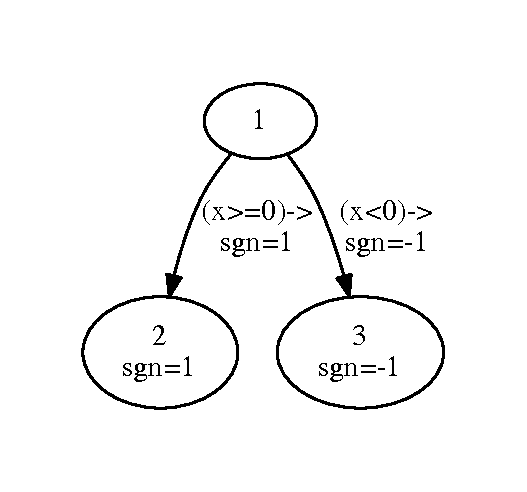
\includegraphics[width=1in,clip=true,trim = 20pt 20pt 30pt 20pt]{figures/sign} \\
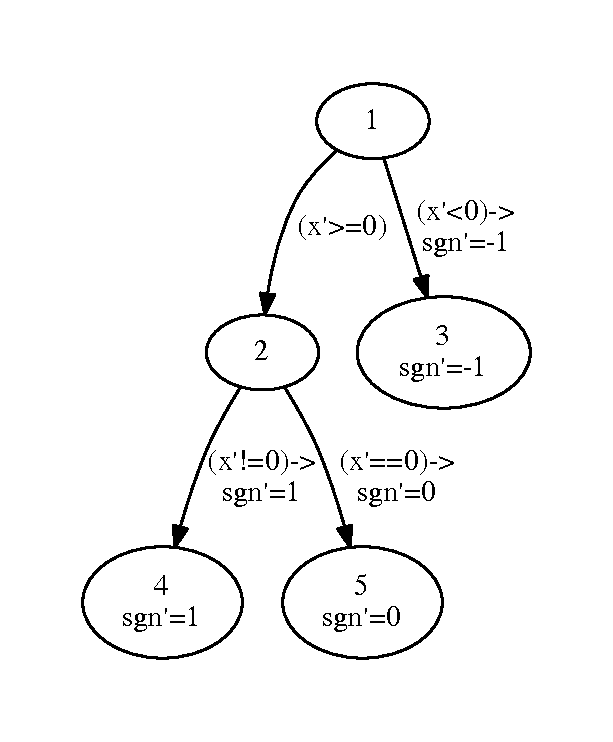
\includegraphics[width=1in,clip=true,trim = 20pt 20pt 30pt 20pt]{figures/sign-tag}
\end{tabular}
\end{minipage}
&
\begin{minipage}[t]{1in}
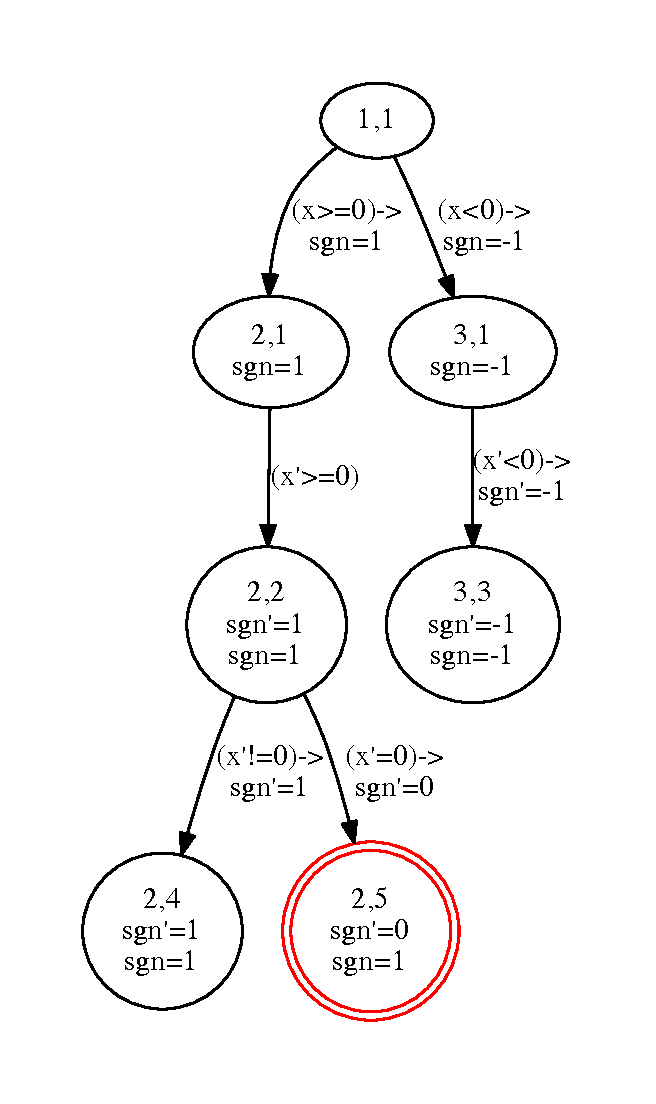
\includegraphics[width=1in,clip=true,trim = 20pt 20pt 30pt 20pt]{figures/sign-correlated}
\end{minipage}
\end{tabular}
\end{figure}


\begin{itemize}
\item $\asemp{v:=e} = l_{\times} \mapsto \{\langle ctx,\asemp{v:=e}_{\A{D}}(data) \rangle | (ctx,data) \in S \}$
\item $\asemp{g:=e} = l_{\times} \mapsto \{\langle \asemp{g:=true}_{\A{D}}(ctx),\asemp{e}_{\A{D}}(data) \rangle  | (ctx,data) \in S \} \cup \{ <\asemp{g:=false}_{\A{D}}(ctx),\asemp{\neg e}_{\A{D}}(data)> | (ctx,data) \in S \}$
\item $\asemp{\textbf{if} (g) \{s_{0}\} \textbf{else} \{s_{1}\}} = l_{\times} \mapsto \{\langle\asemp{g=true}_{\A{D}}(ctx),  \asemp{s_0}_{\A{D}}(data) \rangle | (ctx,data) \in S \} \cup
                                                                                      \{\langle \asemp{g=false}_{\A{D}}(ctx), \asemp{s_1}_{\A{D}}(data) \rangle | (ctx,data) \in S \}$
\item $\asemp{\textbf{goto} lab} = \A{\sigma}$
\end{itemize}
